\begin{answer}

The best $\tau$ in the tests is 0.05, which achieves the least MSE in validation set:

MSE = 0.012400;

With the best $\tau$, the MSE for test set is:

MSE = 0.016990.


Different $\tau$s and their plot. 
\begin{figure}[h]
    \centering
    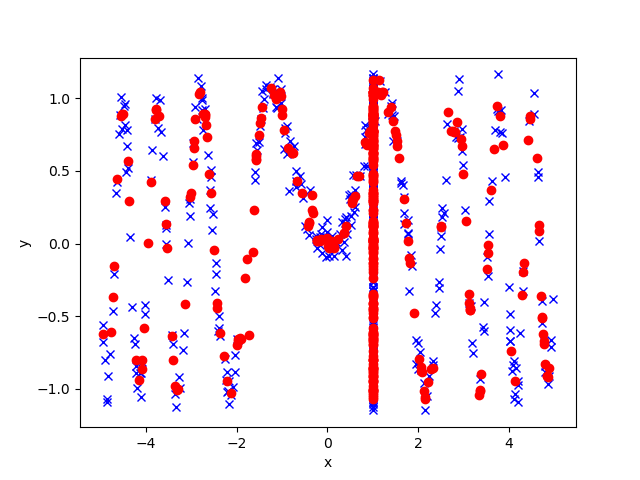
\includegraphics[width=0.6\textwidth]{p05c_pred_0}
    \caption{PS5.c $\tau$=0.030000, MSE = 0.018096}
\end{figure}

\begin{figure}[h]
    \centering
    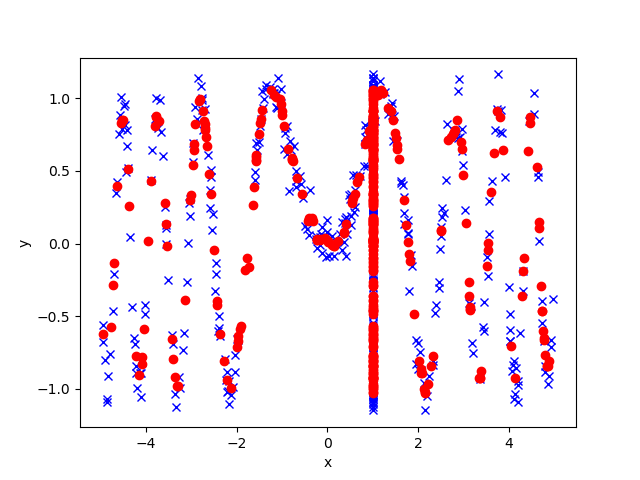
\includegraphics[width=0.6\textwidth]{p05c_pred_1}
    \caption{PS5.c $\tau$=0.050000, MSE = 0.012400, best tau}
\end{figure}

\begin{figure}[h]
    \centering
    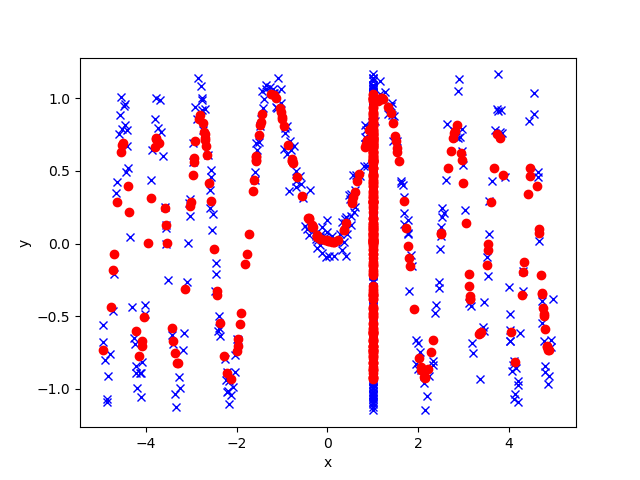
\includegraphics[width=0.6\textwidth]{p05c_pred_2}
    \caption{PS5.c $\tau$=0.100000, MSE = 0.024225}
\end{figure}

\begin{figure}[h]
    \centering
    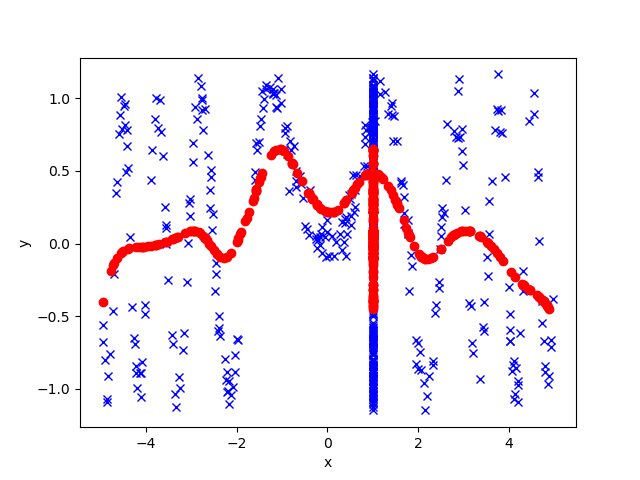
\includegraphics[width=0.6\textwidth]{p05c_pred_3}
    \caption{PS5.c $\tau$=0.500000, MSE = 0.330531}
\end{figure}

\begin{figure}[h]
    \centering
    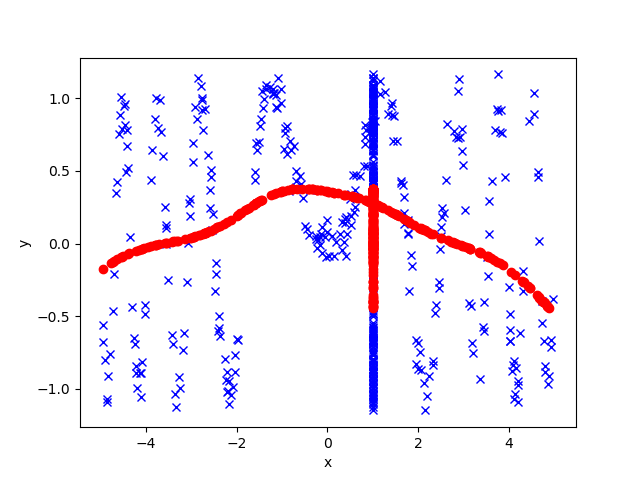
\includegraphics[width=0.6\textwidth]{p05c_pred_4}
    \caption{PS5.c $\tau$=1.000000, MSE = 0.400096}
\end{figure}

\begin{figure}[h]
    \centering
    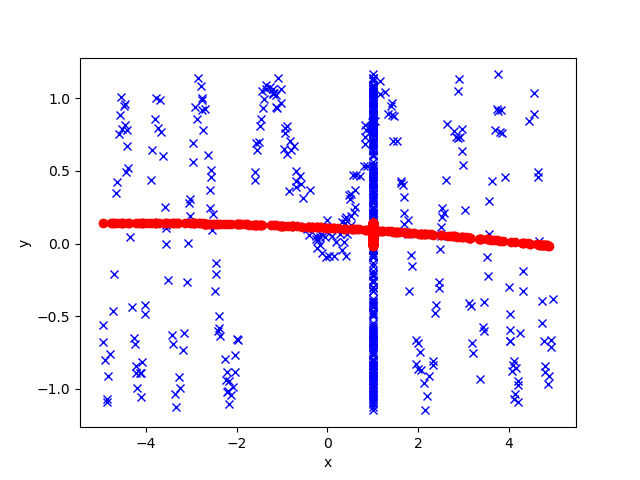
\includegraphics[width=0.6\textwidth]{p05c_pred_5}
    \caption{PS5.c $\tau$=10.000000, MSE = 0.433744}
\end{figure}

\end{answer}
